\documentclass{beamer}
\usepackage{amsmath}
\usepackage{hyperref}
\usepackage{listings}
\usepackage{xcolor}
\hypersetup{colorlinks=true, citecolor=blue, filecolor=blue, linkcolor=blue, urlcolor=blue}
\definecolor{codegreen}{rgb}{0,0.6,0}
\definecolor{codegray}{rgb}{0.5,0.5,0.5}
\definecolor{codepurple}{rgb}{0.58,0,0.82}
\definecolor{backcolour}{rgb}{0.95,0.95,0.92}
 
\lstdefinestyle{mystyle}{
    backgroundcolor=\color{backcolour},   
    commentstyle=\color{codegreen},
    keywordstyle=\color{magenta},
    numberstyle=\tiny\color{codegray},
    stringstyle=\color{codepurple},
    basicstyle=\ttfamily\footnotesize,
    breakatwhitespace=false,         
    breaklines=true,                 
    captionpos=b,                    
    keepspaces=true,                 
    %numbers=left,                    
    numbersep=5pt,                  
    showspaces=false,                
    showstringspaces=false,
    showtabs=false,                  
    tabsize=2
}
 
\lstset{style=mystyle}

\mode<presentation> {

% The Beamer class comes with a number of default slide themes
% which change the colors and layouts of slides. Below this is a list
% of all the themes, uncomment each in turn to see what they look like.

%\usetheme{default}
\usetheme{AnnArbor}
%\usetheme{Antibes}
%\usetheme{Bergen}
%\usetheme{Berkeley}
%\usetheme{Berlin}
%\usetheme{Boadilla}
%\usetheme{CambridgeUS}
%\usetheme{Copenhagen}
%\usetheme{Darmstadt}
%\usetheme{Dresden}
%\usetheme{Frankfurt}
%\usetheme{Goettingen}
%\usetheme{Hannover}
%\usetheme{Ilmenau}
%\usetheme{JuanLesPins}
%\usetheme{Luebeck}
%\usetheme{Madrid}
%\usetheme{Malmoe}
%\usetheme{Marburg}
%\usetheme{Montpellier}
%\usetheme{PaloAlto}
%\usetheme{Pittsburgh}
%\usetheme{Rochester}
%\usetheme{Singapore}
%\usetheme{Szeged}
%\usetheme{Warsaw}

% As well as themes, the Beamer class has a number of color themes
% for any slide theme. Uncomment each of these in turn to see how it
% changes the colors of your current slide theme.

%\usecolortheme{albatross}
%\usecolortheme{beaver}
%\usecolortheme{beetle}
%\usecolortheme{crane}
%\usecolortheme{dolphin}
%\usecolortheme{dove}
%\usecolortheme{fly}
%\usecolortheme{lily}
%\usecolortheme{orchid}
%\usecolortheme{rose}
%\usecolortheme{seagull}
%\usecolortheme{seahorse}
%\usecolortheme{whale}
%\usecolortheme{wolverine}

%\setbeamertemplate{footline} % To remove the footer line in all slides uncomment this line
\setbeamertemplate{footline}[page number] % To replace the footer line in all slides with a simple slide count uncomment this line

\setbeamertemplate{navigation symbols}{} % To remove the navigation symbols from the bottom of all slides uncomment this line
}

\usepackage{graphicx} % Allows including images
\usepackage{booktabs} % Allows the use of \toprule, \midrule and \bottomrule in tables
%\usepackage {tikz}
\usepackage{tkz-graph}
\GraphInit[vstyle = Shade]
\tikzset{
  LabelStyle/.style = { rectangle, rounded corners, draw,
                        minimum width = 2em, fill = yellow!50,
                        text = red, font = \bfseries },
  VertexStyle/.append style = { inner sep=5pt,
                                font = \normalsize\bfseries},
  EdgeStyle/.append style = {->, bend left} }
\usetikzlibrary {positioning}
%\usepackage {xcolor}
\definecolor {processblue}{cmyk}{0.96,0,0,0}
%----------------------------------------------------------------------------------------
%	TITLE PAGE
%----------------------------------------------------------------------------------------

\title[Gradient Descent]{Numerical Optimization V: 1st order methods} %

\author{Qiang Zhu} % Your name
\institute[University of Nevada Las Vegas] % Your institution as it will appear on the bottom of every slide, may be shorthand to save space
{
University of Nevada Las Vegas\\ % Your institution for the title page
\medskip
}
\date{\today} % Date, can be changed to a custom date

\begin{document}

\begin{frame}
\titlepage % Print the title page as the first slide
\end{frame}

\begin{frame}
\frametitle{Overview} % Table of contents slide, comment this block out to remove it
\tableofcontents % Throughout your presentation, if you choose to use \section{} and \subsection{} commands, these will automatically be printed on this slide as an overview of your presentation
\end{frame}

%----------------------------------------------------------------------------------------
%	PRESENTATION SLIDES
%----------------------------------------------------------------------------------------

%------------------------------------------------

\section{In choosing the direction}
\begin{frame}{The choice of descent direction}
In the previous chapter, we have talked about the general strategy for optimization is to decide a direction and then use the line search method to obtain a sufficient decrease. Repeating it for many time, we expect to arrive at the local minimum.
\begin{equation*}
    x^{k+1} = x^k + \alpha^k d^k
\end{equation*} 
The search direction often has the form
\begin{equation}
    d^k = -B^k^{-1} \nabla f(x^k)
\end{equation}

where $B^k$ is a symmetric and nonsingular matrix. In some method (e.g., steepest descent), $B^k$ is the identify matrix, while in (quasi-) Newton's method, $B&k$ is the approximate or exact Hessian. 

In this lecture, we will cover the \textcolor{blue}{first-order} methods which \textcolor{blue}{purely rely on the gradient information}.

\end{frame}

\section{Gradient Descent}
\begin{frame}{Gradient descent}
An intuitive choice for the descent direction is the direction of steepest descent ($g^k = \nabla f(x^k)$).
\begin{equation*}
    d^k = - \frac{g^k}{||g^k||}
\end{equation*}

If we optimize the step size at each step, we have
\begin{equation*}
    \alpha^k = \underset{\alpha}{\arg \min} f(x^k + \alpha d^k)
\end{equation*}

Since 
\begin{equation*}
    \nabla f(x^k + \alpha d^k)^T d^k = 0
\end{equation*}
We know
\begin{equation*}
    d^{k+1} = - \frac{\nabla f(x^k + \alpha d^k)}{||\nabla f(x^k + \alpha^k)||}
\end{equation*}
It is obvious that the two consecutive directions are \textcolor{blue}{orthogonal}.
\begin{equation*}
    d^{k+1}^T d^k = 0
\end{equation*}

\end{frame}

\section{Conjugate gradient}
\begin{frame}{Conjugate gradient}
Gradient descent can perform poorly in narrow valleys. The conjugate gradient method overcomes this issue by doing a small transformation.

When minimizing the quadratic functions:
\begin{equation*}
    \underset{\alpha}{\textrm{minimize}}: f(x) = \frac{1}{2} x^T A x - b^T x 
\end{equation*}

is equivalent to solving the linear equation
\begin{equation*}
    Ax = b
\end{equation*}
where $A$ is $N \times N$ symmetric and positive definite, and thus $f$ has a unique local minimum.

When solving $Ax = b$, a powerful method is to find a sequence of $N$ \textcolor{blue}{conjugate directions} satisfying 
\begin{equation*}
    d^i^T A d^j = 0 ~~~ (i\neq j)
\end{equation*}

\end{frame}

\begin{frame}{To find the successive conjugate directions}
One can start with the direction of steepest descent
    \begin{equation*}
        d^1 = - g^1
    \end{equation*}
We then use line search to find the next design point. For quadratic functions $f= \frac{1}{2} x^T A x - b^T x $, the step factor $\alpha$ can be computed as
\begin{equation*}
\begin{split}
    \frac{\partial f(x+\alpha d)}{\partial \alpha} & = \frac{\partial}{\partial\alpha} \Bigg[\frac{1}{2} (x+\alpha d)^T A (x+\alpha d) + b^T (x+\alpha d) + c \Bigg]\\
    & = d^T A(x + \alpha d) + d^T b\\
    & = d^T(Ax + b) + \alpha d^T A d
\end{split}
\end{equation*}
Let the gradient be zero, 
\begin{equation*}
    \alpha = - \frac{d^T(Ax + b)}{d^T A d}
\end{equation*}

Then the update is
\begin{equation*}
    x^2 = x^1 + \alpha d^1
\end{equation*}

\end{frame}

\begin{frame}{To find the successive conjugate directions (continued)}
For the next step
    \begin{equation*}
        d^{k+1} = -g^{k+1} + \beta^k d^k
    \end{equation*}
where $\beta^k$ is a series of scalar parameters. Larger values of $\beta$ indicate that the previous descent direction contributes strongly.

We solve $\beta$, from the followings
\begin{gather*}
    d^{(k+1)T} A d^k = 0 \\
    (-g^{k+1} + \beta^k d^{(k)})^T A d^{(k)} = 0\\
    -g^{k+1}A d^{(k)} + \beta^k d^{(k)T} A d^{(k)} = 0 \\
    \beta^k = \frac{g^{(k+1)T}A d^{(k)}}{d^{(k)T}A d^{(k)}} 
\end{gather*}
The conjugate method is exact for quadratic functions. But it can be applied to non quadractic functions as well when the quadratic function is a good approximation.

\end{frame}

\begin{frame}{To Approximate $A$ and $\beta$}
Unfortunately, we don't know the value of $A$ that best approximate $f$ around $x^k$. So we choose some way to compute $\beta$.

\begin{alertblock}{Fletcher-Reeves}
\begin{equation*}
    \beta^k = \frac{g^{(k)T} g^{(k)}}{g^{(k-1)T} g^{(k-1)}}
\end{equation*}
\end{alertblock}
\vfill
\begin{alertblock}{Polak-Ribiere}
\begin{equation*}
    \beta^k = \frac{g^{(k)T} (g^{(k)}-g^{(k-1)})}{g^{(k-1)T} g^{(k-1)}}
\end{equation*}
\end{alertblock}

\end{frame}


\begin{frame}{Comparison between Conjugate Gradient and Steepest Descent}
\begin{figure}
\centering
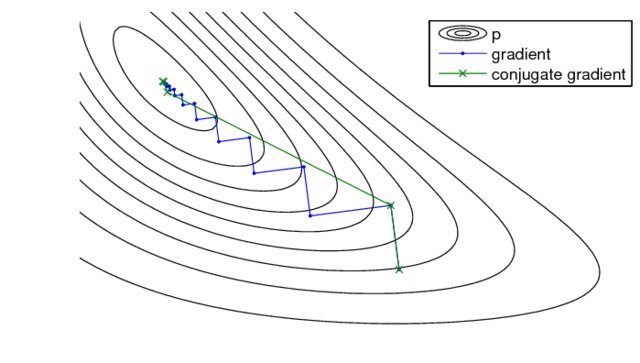
\includegraphics[width=120mm]{Lecture_notes/Figs/cg-sd.jpg}
\end{figure}
\end{frame}



\section{Summary}
\begin{frame}{Summary}
    \begin{itemize}
        \item Gradient descent follows the direction of steepest descent
        \item Two consecutive search directions in gradient descent are orthogonal
        \item In conjugate gradient, the search directions are conjugate with respect to an approximate hessian.
        \item Both SD and CG work with the line search method
    \end{itemize}
\end{frame}
\end{document}

